\documentclass[]{article}
\usepackage[UTF8]{ctex}
\usepackage[a4paper,left=10mm,right=10mm,bottom=10mm,top=10mm]{geometry}
\usepackage{graphicx}
\usepackage{float}
\usepackage{amsmath,amsfonts,amssymb,amsthm}
\usepackage{array,color}
%opening
\title{计算机科学中的数学基础Exercise9}
\author{陈昱衡 521021910939}
\date{\today}

\begin{document}

\maketitle


\section*{Warmup1}
\begin{figure}[H]
    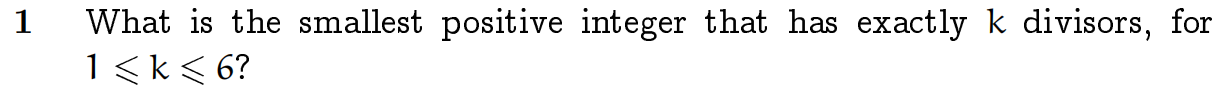
\includegraphics[scale = 0.6]{2023-03-13-16-09-17.png}
\end{figure}
分别是1,2,4,6,16,18.


\section*{Warmup2}
\begin{figure}[H]
    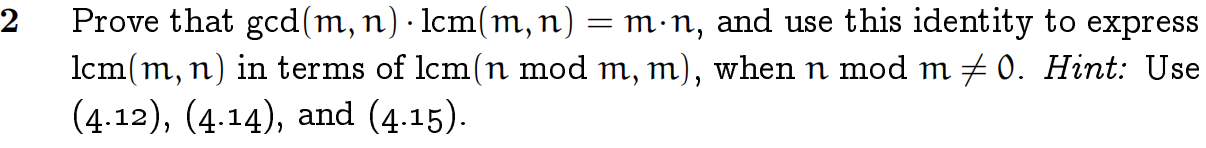
\includegraphics[scale = 0.6]{2023-03-13-16-11-00.png}
\end{figure}
由4.14,
\begin{align}
    k &= gcd(m,n) \Leftrightarrow k_{p} = min(m_{p} , n_{p})\quad,for\quad any\quad p\\
    k &= lcm(m,n) \Leftrightarrow k_{p} = max(m_{p} , n_{p})\quad,for\quad any\quad p
\end{align}
故,
\begin{align}
    gcd(m,n) \times lcm(m,n) \Leftrightarrow k_{p} = min(m_{p},n_{p}) + max(m_{p},n_{p}) \quad,for\quad any\quad p\\
    \Leftrightarrow k_{p} = m_{p} + n_{p} \quad for\quad any\quad p\\
\end{align}
因为$m + n = max(m,n)+min(m,n)$,
所以,
\begin{align}
    m \times n &\Leftrightarrow k_{p} = m_{p} + n_{p} \quad for\quad any\quad p\\
    gcd(m,n) \times lcm(m,n) &= m \times n
\end{align}

\section*{Warmup3}
\begin{figure}[H]
    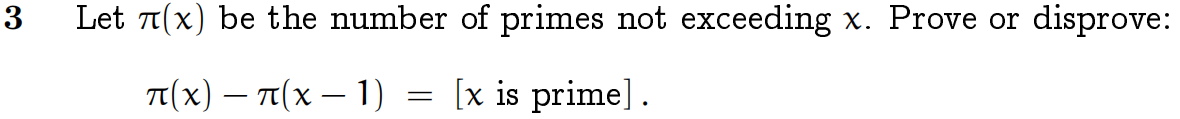
\includegraphics[scale = 0.6]{2023-03-13-16-11-22.png}
\end{figure}
显然对于整数,该式成立,因为 $\pi$(x)与$\pi$(x-1)的差取决于x是否为素数.\par 
对于x为实数的情况,显然,借助向下取整函数,$\pi$(x)=$\pi$($\lfloor x\rfloor$),因此,实数的情形可以转化为整数的情况,
\begin{equation}
    \pi(x) - \pi(x-1) = [\lfloor x \rfloor \quad is \quad prime]
\end{equation}


\section*{Basics14}
\begin{figure}[H]
    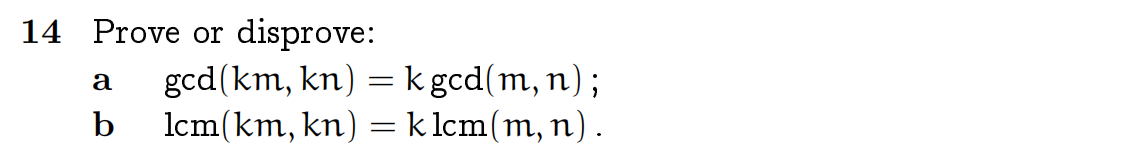
\includegraphics[scale = 0.6]{2023-03-13-16-11-35.png}
\end{figure}
结论:当k为非负整数时,该式成立.\par 
首先,由式4-14,4-15,有
\begin{align}
    gcd(m,n) &= \prod_{p}^{}p^{min(m_{p},n_{p})}\\
    lcm(m,n) &= \prod_{p}^{}p^{max(m_{p},n_{p})}
\end{align}
而k也可以表示为$\langle k_{1},k_{2},\cdots  \rangle$,即$\prod_{p}^{}p^{k_{p}}$。
设$km=m^{'},kn=n^{'}$,则有:
\begin{align}
    gcd(m^{'},n^{'}) &= \prod_{p}^{}p^{min(m^{'}_{p},n^{'}_{p})}\\
    lcm(m^{'},n^{'}) &= \prod_{p}^{}p^{max(m^{'}_{p},n^{'}_{p})}\\
    m^{'}_{p} &= k_{p} + m_{p}\\
    n^{'}_{p} &= k_{p} + n_{p}
\end{align}
从而,
\begin{align}
    gcd(m^{'},n^{'}) &= \prod_{p}^{}p^{min(m^{'}_{p},n^{'}_{p})}\\
                    &= \prod_{p}^{}p^{min(m_{p},n_{p}) + k_{p}} \\
                    &=\prod_{p}^{}p^{min(m_{p},n_{p})} \times k \\
    lcm(m^{'},n^{'}) &= \prod_{p}^{}p^{max(m^{'}_{p},n^{'}_{p})} \\
                    &= \prod_{p}^{}p^{max(m_{p},n_{p}) + k_{p}} \\
                    &=\prod_{p}^{}p^{max(m_{p},n_{p})} \times k 
\end{align}
即,
\begin{align}
    gcd(km,kn) &= \prod_{p}^{}p^{min(m_{p},n_{p})} \times k \\
    lcm(km,kn) &=\prod_{p}^{}p^{max(m_{p},n_{p})} \times k 
\end{align}

\section*{Basics15}
\begin{figure}[H]
    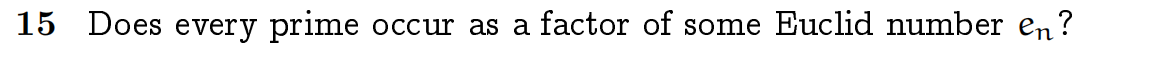
\includegraphics[scale =0.6]{2023-03-13-16-11-46.png}
\end{figure}
不是,由欧拉数的定义,显然可以看出,
\begin{align}
    e_{1} &=2\\
    e_{2} &=3\\
    e_{3} &=7\\
    e_{4} &=43\\
\end{align}
    因此,我们可以假设欧拉数 e (mod 5) = 2 或 3.
\par 
若欧拉数$e_{n-1}(mod5) = 2$,有$e_{n} = e_{n-1} \times (e_{n-1} - 1) = (5k + 2)\times(5k+1) + 1 = 25k^2+15k+3$,则$e_{n}(mod 5) = 3$,
若欧拉数$e_{n-1}(mod5) = 3$,有$e_{n} = e_{n-1} \times (e_{n-1} - 1) = (5k + 3)\times(5k+2) +1= 25k^2+15k+7$,则$e_{n}(mod 5) = 2$,
故,可以从2开始使用数学归纳法。
\end{document}